%%
% TUM report for the individual assignment in
% Business Process Prediction, Simulation, and Optimization.
%%

\documentclass[
  english,
  font=times,
  twocolumn,
]{tumarticle}

\usepackage{cite}
\usepackage{booktabs}
\usepackage{array}
\usepackage{graphicx}
\usepackage{tabularx}

\setlength{\tabcolsep}{4pt}
\renewcommand{\arraystretch}{1.12}
\makeatletter
\let\oldthebibliography\thebibliography
\let\endoldthebibliography\endthebibliography
\renewenvironment{thebibliography}[1]
  {\oldthebibliography{#1}\small\raggedright\setlength{\itemsep}{0.15em}}
  {\endoldthebibliography}
\makeatother

\title{First Assignment - Business Process Prediction, Simulation, and Optimization - Summer Semester 2026}
\subtitle{Process and Data Science on the BPIC-17 Event Log}

\author[email=15500841929.zhang@tum.de]{Jianguo Zhang}
\date{\today}

\begin{document}

\maketitle

\begin{abstract}
This report analyzes the BPIC-17 event log of a Dutch financial institution's loan application process using reproducible Python-based process mining.
The log contains 31,509 cases, 1,202,267 events, and 15,930 process variants, which already indicates substantial behavioral diversity.
Process discovery and conformance checking show that a Heuristics Miner model gives the most useful final trade-off for simulation-oriented analysis, with fitness 0.834, precision 0.998, and generalization 0.848 on the complete-event log.
Decision mining identifies data-aware branching behavior around application validation and returned offers, while the advanced duration-prediction analysis shows only modest improvement over a median baseline, suggesting that early-case information alone has limited predictive power.
\end{abstract}

\section{Introduction}

The BPIC-17 event log records a loan application process at a Dutch financial institution and was released for the BPI Challenge 2017 \cite{bpichallenge2017}.
It captures interactions among application, offer, and workflow activities, including case attributes such as loan goal, application type, and requested amount.
The analysis goal is to move from descriptive event log inspection to a process model that can support later prediction, simulation, and optimization tasks.
All code and generated intermediate results are available in the public repository\footnote{\url{https://github.com/shifuyoubanfa/bpic-2017-process-mining-assignment}}; the raw XES file is intentionally excluded from version control.

\section{Approach and Results}

\subsection{Technical Setup and Preliminaries}

The analysis was implemented in Python\footnote{\url{https://www.python.org/}} with pandas\footnote{\url{https://pandas.pydata.org/}}, NumPy\footnote{\url{https://numpy.org/}}, PM4Py\footnote{\url{https://pm4py.fit.fraunhofer.de/}} \cite{pm4py}, matplotlib\footnote{\url{https://matplotlib.org/}}, scikit-learn\footnote{\url{https://scikit-learn.org/}}, Jupyter\footnote{\url{https://jupyter.org/}}, and Graphviz\footnote{\url{https://graphviz.org/}}.
The reproducible environment is documented in \texttt{requirements.txt} and \texttt{environment.yml}.
All notebooks use relative project paths, and the random seed is fixed to 42 for sampling and train-test splits.
The event log was read from \texttt{data/BPI Challenge 2017.xes}; this local data file is ignored by Git to avoid publishing the raw event log.

\subsection{Simple Event Log Analysis}

Table \ref{tab:logstats} summarizes the required descriptive statistics.
The log is large and behaviorally diverse: 31,509 loan applications produce more than 1.2 million events and 15,930 variants.
Cases contain 38.16 events on average, but the maximum case length is 180 events.
The average throughput time is 21.90 days, while the maximum duration reaches 286.07 days, which indicates that some applications remain open far longer than the typical case.

\begin{table}[t]
    \caption{Basic event log statistics.}
    \centering
    \small
    \begin{tabular}{lr}
        \toprule
        \textbf{Metric} & \textbf{Value} \\
        \midrule
        Cases & 31,509 \\
        Events & 1,202,267 \\
        Process variants & 15,930 \\
        Activities & 26 \\
        Resources & 149 \\
        Case attributes & 3 \\
        Event attributes & 15 \\
        Categorical event attributes & 9 \\
        Mean case length & 38.16 \\
        Std. case length & 16.72 \\
        Mean duration days & 21.90 \\
        Std. duration days & 13.17 \\
        Mean duration minutes & 31,535.43 \\
        Mean duration seconds & 1,892,125.92 \\
        \bottomrule
    \end{tabular}
    \label{tab:logstats}
\end{table}

Two additional descriptive statistics are useful for interpretation.
First, workflow events dominate the log with 768,823 events, followed by application events (239,595) and offer events (193,849).
Second, the most frequent loan goals are car loans (9,328 cases), home improvement (7,669), and existing loan takeover (5,601).
The high number of variants and long-running cases suggest that a useful simulation base model must balance replay behavior against simplicity rather than maximize only one quality metric.

\subsection{Process Model Creation and Validation}

Before discovery, the lifecycle distribution was inspected.
Only 475,306 of the 1,202,267 events have \texttt{lifecycle:transition = complete}; the remaining events describe scheduling, starting, suspending, resuming, aborting, or withdrawing workflow tasks.
The final discovery input therefore uses complete events, because they best represent completed business activities and reduce task-lifecycle noise.
The risk is that start, schedule, suspend, resume, and withdraw information is removed; this choice was documented by saving both the lifecycle distribution and the \texttt{EventOrigin} by lifecycle crosstab.

Three discovery algorithms were evaluated using the standard quality dimensions of fitness, precision, generalization, and simplicity \cite{vanderAalst2016process,carmona2018conformance}: Inductive Miner, Heuristics Miner, and Alpha Miner.
Inductive Miner provides a structured and perfectly fitting model, but its low precision indicates over-generalization for this log.
Alpha Miner is useful only as a baseline because the real-life log is noisy and highly variable.
Heuristics Miner is selected as the final process model because it replays approximately the target share of cases while preserving very high precision and acceptable generalization.

\begin{table*}[t]
    \caption{Process model quality metrics on the complete-event full log.}
    \centering
    \small
    \begin{tabular}{lrrrrrrrr}
        \toprule
        \textbf{Model} & \textbf{Fitness} & \textbf{Precision} & \textbf{General.} & \textbf{Simplicity} & \textbf{Places} & \textbf{Trans.} & \textbf{Arcs} & \textbf{Silent ratio} \\
        \midrule
        Inductive Miner & 1.000 & 0.293 & 0.976 & 0.617 & 34 & 53 & 114 & 0.547 \\
        Heuristics Miner & 0.834 & 0.998 & 0.848 & 0.481 & 49 & 94 & 220 & 0.745 \\
        Alpha Miner & 0.496 & 0.126 & 0.987 & 0.392 & 25 & 24 & 87 & 0.000 \\
        \bottomrule
    \end{tabular}
    \label{tab:modelquality}
\end{table*}

The final BPMN 2.0 model is derived from the Heuristics Miner Petri net and exported as both BPMN XML and PDF.
The model prioritizes precision and simulation usefulness: it avoids the overly permissive behavior of the Inductive Miner, while still replaying 83.4\% of the complete-event log.
Its main limitation is structural complexity, visible in its 49 places, 94 transitions, 220 arcs, and high silent-transition ratio.
Additional discovered models are included in the appendix to make the algorithm comparison transparent.

\begin{figure*}[t]
    \centering
    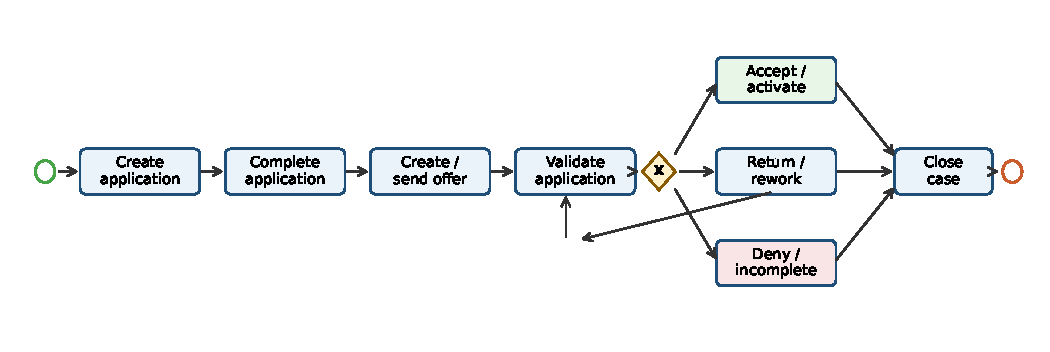
\includegraphics[width=.94\textwidth]{../figures/process_models/final_heuristics_bpmn_report.pdf}
    \caption{Readable final BPMN 2.0-style view derived from the selected Heuristics Miner model. The full exported BPMN model is provided in the appendix.}
    \label{fig:finalbpmn}
\end{figure*}

\subsection{Decision Mining}

Decision mining was performed on the complete-event log using branching activities as candidate decision points \cite{deleoni2013decision}.
The selected points are \texttt{A\_Validating}, with 38,813 instances and six grouped successor classes, and \texttt{O\_Returned}, with 23,303 instances and six grouped successor classes.
Features were restricted to information available before the decision: case attributes, requested amount, elapsed time, prefix length, previous activity, activity counts, and event-origin counts.
This avoids future leakage and makes the resulting decision rules meaningful for simulation.

\begin{table}[t]
    \caption{Decision mining performance.}
    \centering
    \small
    \begin{tabular}{llrr}
        \toprule
        \textbf{Point} & \textbf{Model} & \textbf{Acc.} & \textbf{Macro F1} \\
        \midrule
        \texttt{A\_Validating} & Tree & 0.567 & 0.267 \\
        \texttt{A\_Validating} & Forest & 0.668 & 0.346 \\
        \texttt{O\_Returned} & Tree & 0.214 & 0.257 \\
        \texttt{O\_Returned} & Forest & 0.354 & 0.369 \\
        \bottomrule
    \end{tabular}
    \label{tab:decisionmetrics}
\end{table}

The decision trees are the main explanatory artifacts, while random forests are used as a performance comparison and for feature importance.
For \texttt{A\_Validating}, important features include the number of previous application-origin events, repeated validation and incomplete behavior, elapsed time, prefix length, and requested amount.
For \texttt{O\_Returned}, the previous activity and prior incomplete behavior are especially informative.
Performance is limited by class imbalance and by grouping rare successors into an \texttt{Other} class, but the rules still identify data attributes that can parameterize XOR routing in a simulation model.

\begin{center}
    \begin{minipage}{.98\columnwidth}
        \centering
        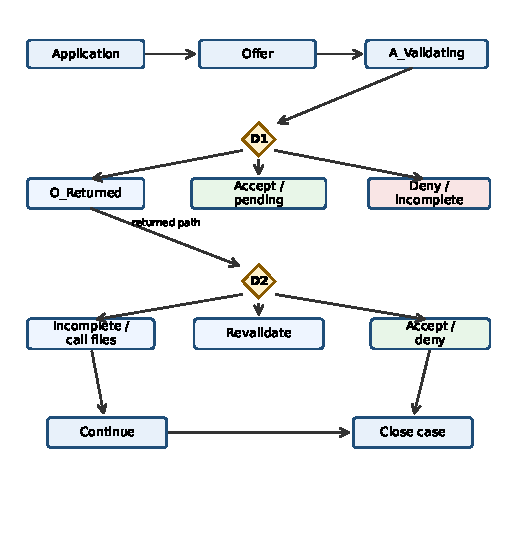
\includegraphics[width=.96\linewidth]{../figures/process_models/final_decision_aware_bpmn_report.pdf}
        \captionof{figure}{Decision-aware BPMN-style view with mined decision blocks for the two selected XOR decisions.}
        \label{fig:decisionaware}
    \end{minipage}
\end{center}

\subsection{Advanced Analysis}

The advanced analysis asks whether early case behavior can predict remaining loan-application duration.
The hypothesis is that case attributes and the first five complete events contain enough information to improve remaining-time estimates compared with a median baseline.
This is relevant for simulation and optimization because a calibrated duration model can support workload forecasting, prioritization, and what-if experiments.

The prediction dataset contains 31,509 eligible cases; 22,056 were used for training and 9,453 for testing.
The target is remaining duration in days after the fifth complete event.
The random forest regressor improves over the median baseline, but only modestly: MAE decreases from 10.13 to 9.95 days, RMSE decreases from 12.77 to 12.12 days, and $R^2$ increases from -0.079 to 0.030.
Elapsed time is the most important feature, followed by requested amount and application type.
The result suggests that early-case information has some predictive value, but it is insufficient for accurate individual-case forecasting without later process behavior or richer contextual data.

\begin{table}[t]
    \caption{Remaining duration prediction after five complete events.}
    \centering
    \small
    \begin{tabular}{lrrr}
        \toprule
        \textbf{Model} & \textbf{MAE} & \textbf{RMSE} & \textbf{$R^2$} \\
        \midrule
        Median baseline & 10.13 & 12.77 & -0.079 \\
        Random forest & 9.95 & 12.12 & 0.030 \\
        \bottomrule
    \end{tabular}
    \label{tab:advancedmetrics}
\end{table}

\section{Discussion and Conclusion}

The analyses show that BPIC-17 is large, highly variable, and rich enough for data-aware process mining.
For simulation, the selected Heuristics Miner model is preferable to the Inductive Miner because it avoids excessive behavior while still replaying around 80\% of the complete-event log.
The decision mining results identify plausible routing variables, but the measured predictive performance also shows that the decision points are not fully explained by the available case and prefix features.
The duration-prediction experiment gives a similar message: early information helps only slightly, so future simulation work should incorporate later event updates, resource availability, and possibly queueing or workload features.

\section{Usage Declaration}

Open-source tools used in the project are listed in the technical setup section.
Generative AI assistance was used to help structure the repository, draft reproducible code, and prepare the report text.
All numerical results, figures, and claims in this report were checked against the repository outputs, and responsibility for the submitted content remains with the author.
No commercial process mining tool was used.

\FloatBarrier
\bibliographystyle{unsrt}
\bibliography{references}

\clearpage
\appendix

\section{Supplementary Figures}

\begin{figure*}[p]
    \centering
    
\includegraphics[width=.92\textwidth]{../figures/process_models/final_heuristics_bpmn.pdf}
    \caption{Full exported BPMN model derived from the selected Heuristics Miner model.}
    \label{fig:fullfinalbpmn}
\end{figure*}

\begin{figure*}[p]
    \centering
    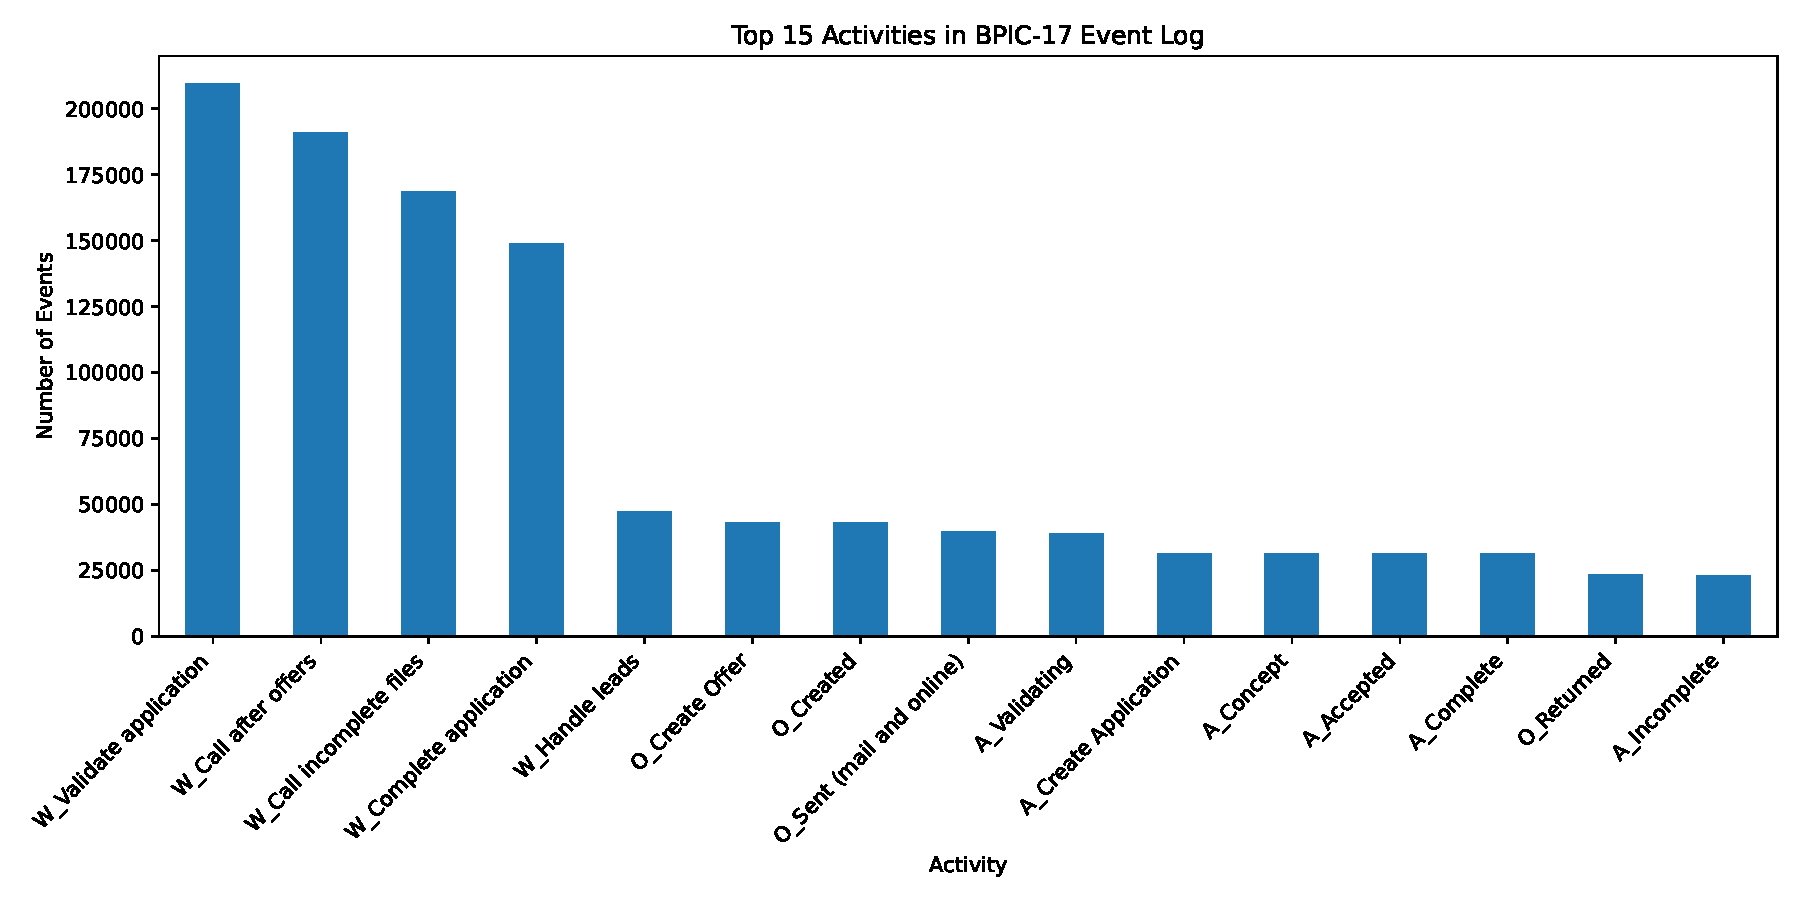
\includegraphics[width=.92\textwidth]{../figures/top_15_activities.pdf}
    \caption{Top 15 activity frequencies.}
    \label{fig:topactivities}
\end{figure*}

\begin{figure*}[p]
    \centering
    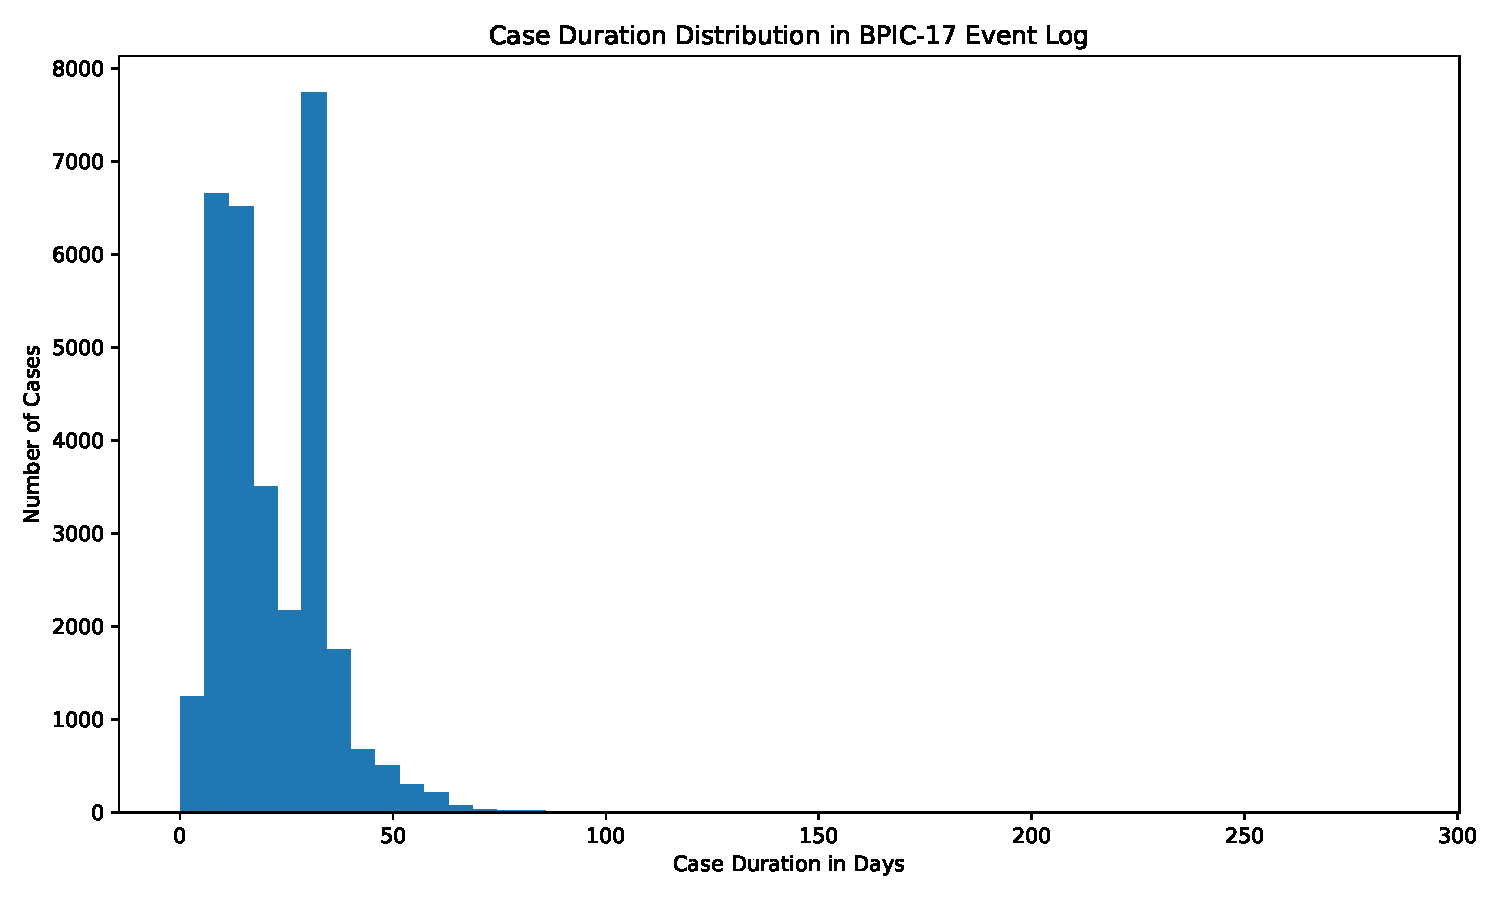
\includegraphics[width=.92\textwidth]{../figures/case_duration_distribution_days.pdf}
    \caption{Case duration distribution in days.}
    \label{fig:durationdist}
\end{figure*}

\begin{figure*}[p]
    \centering
    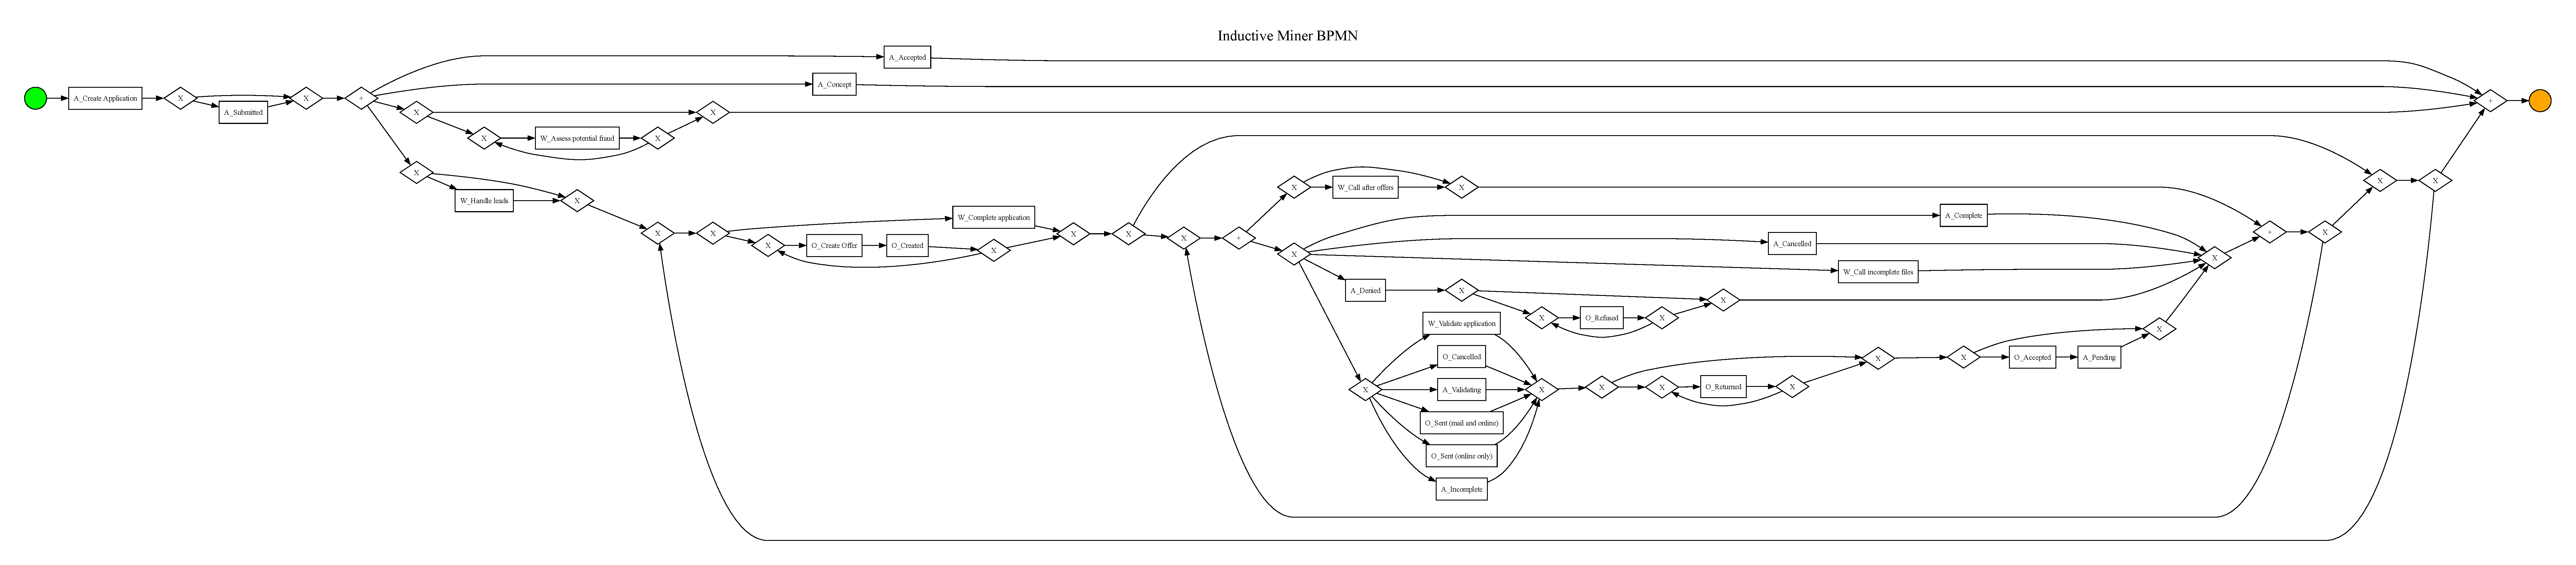
\includegraphics[width=.92\textwidth]{../figures/process_models/inductive_miner_bpmn.pdf}
    \caption{Inductive Miner BPMN model.}
    \label{fig:inductivebpmn}
\end{figure*}

\begin{figure*}[p]
    \centering
    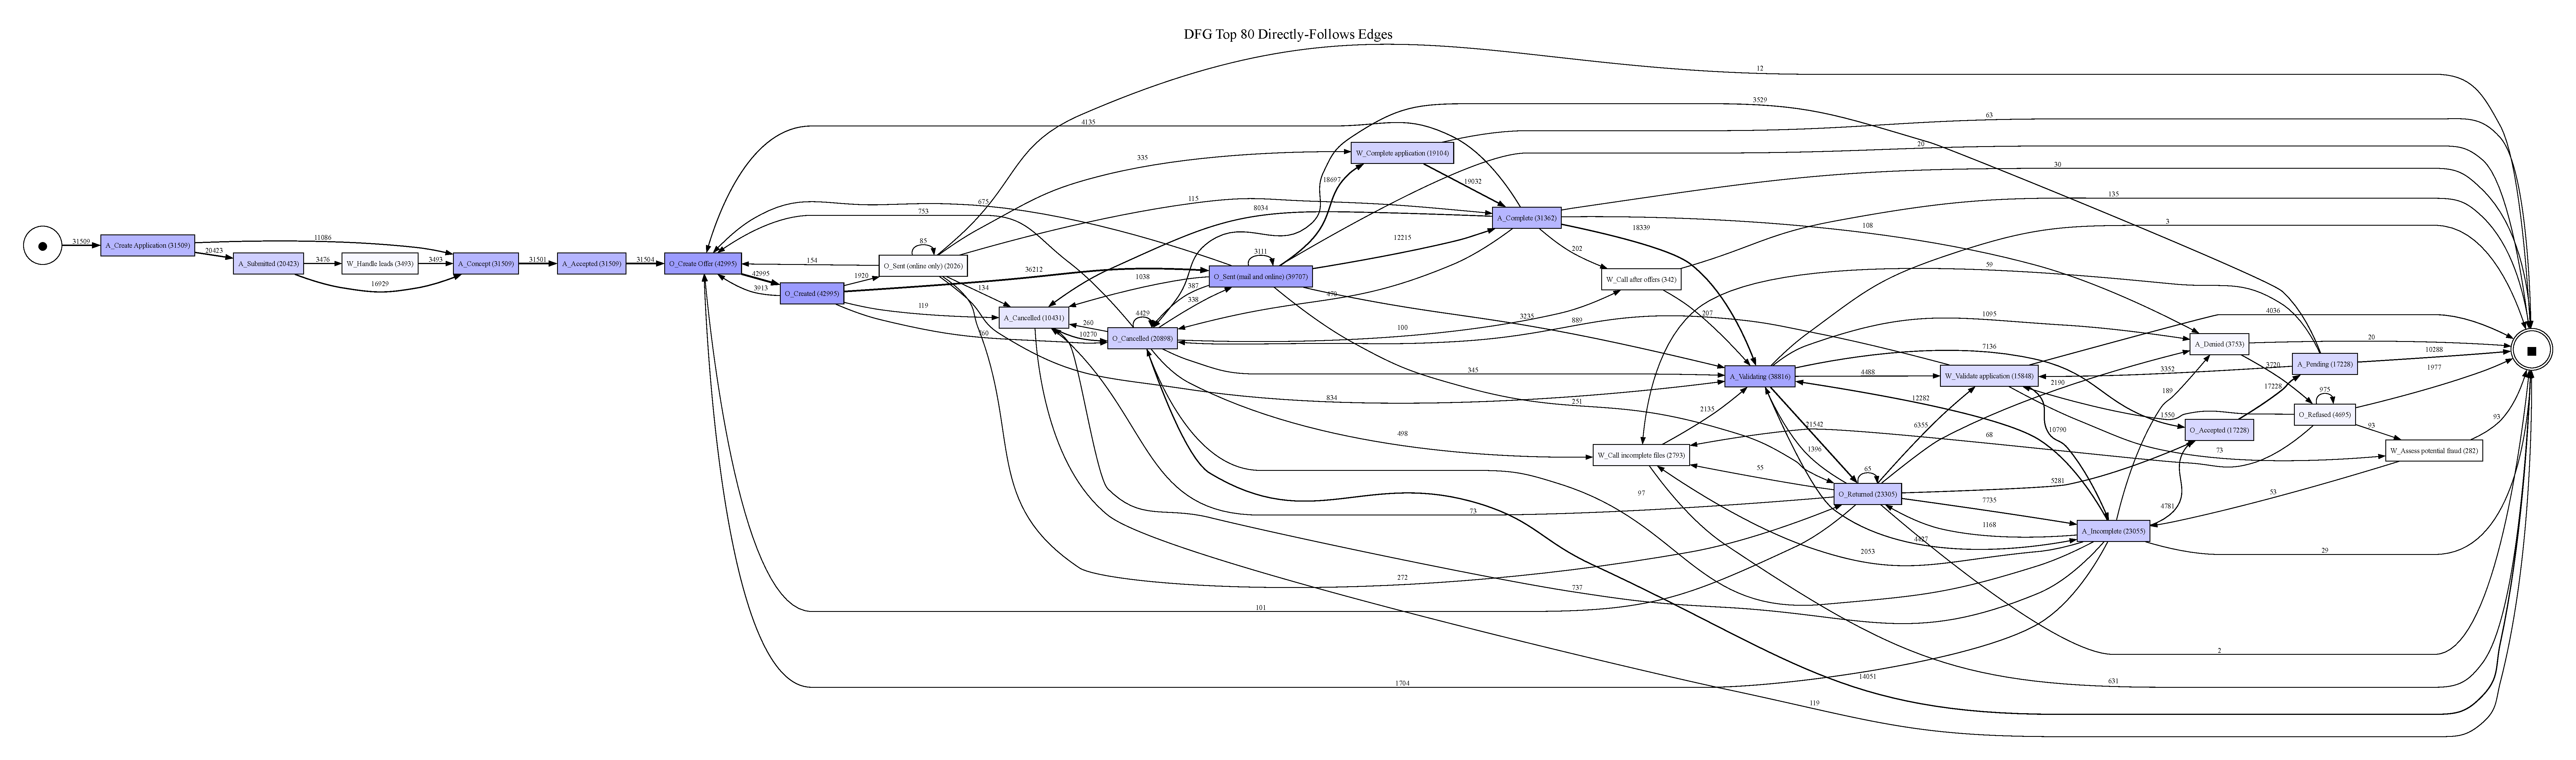
\includegraphics[width=.92\textwidth]{../figures/process_models/dfg_top_edges.pdf}
    \caption{Top directly-follows graph edges.}
    \label{fig:dfg}
\end{figure*}

\begin{figure*}[p]
    \centering
    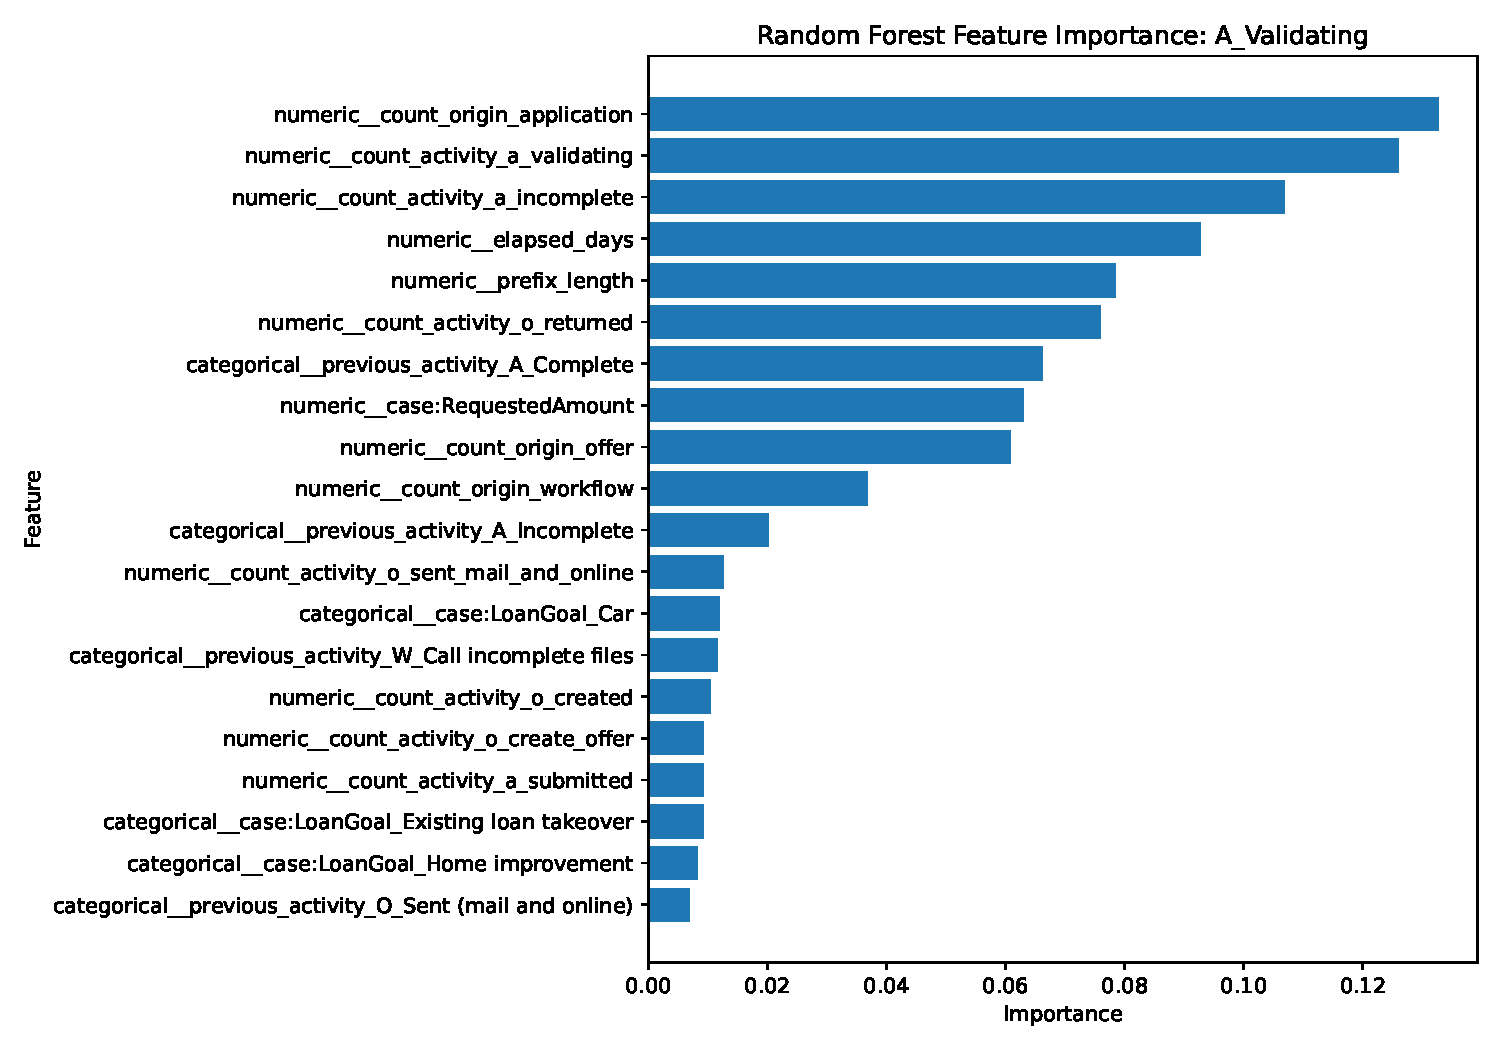
\includegraphics[width=.92\textwidth]{../figures/decision_mining/feature_importance_a_validating.pdf}
    \caption{Feature importance for the \texttt{A\_Validating} decision point.}
    \label{fig:avalidatingfeatures}
\end{figure*}

\begin{figure*}[p]
    \centering
    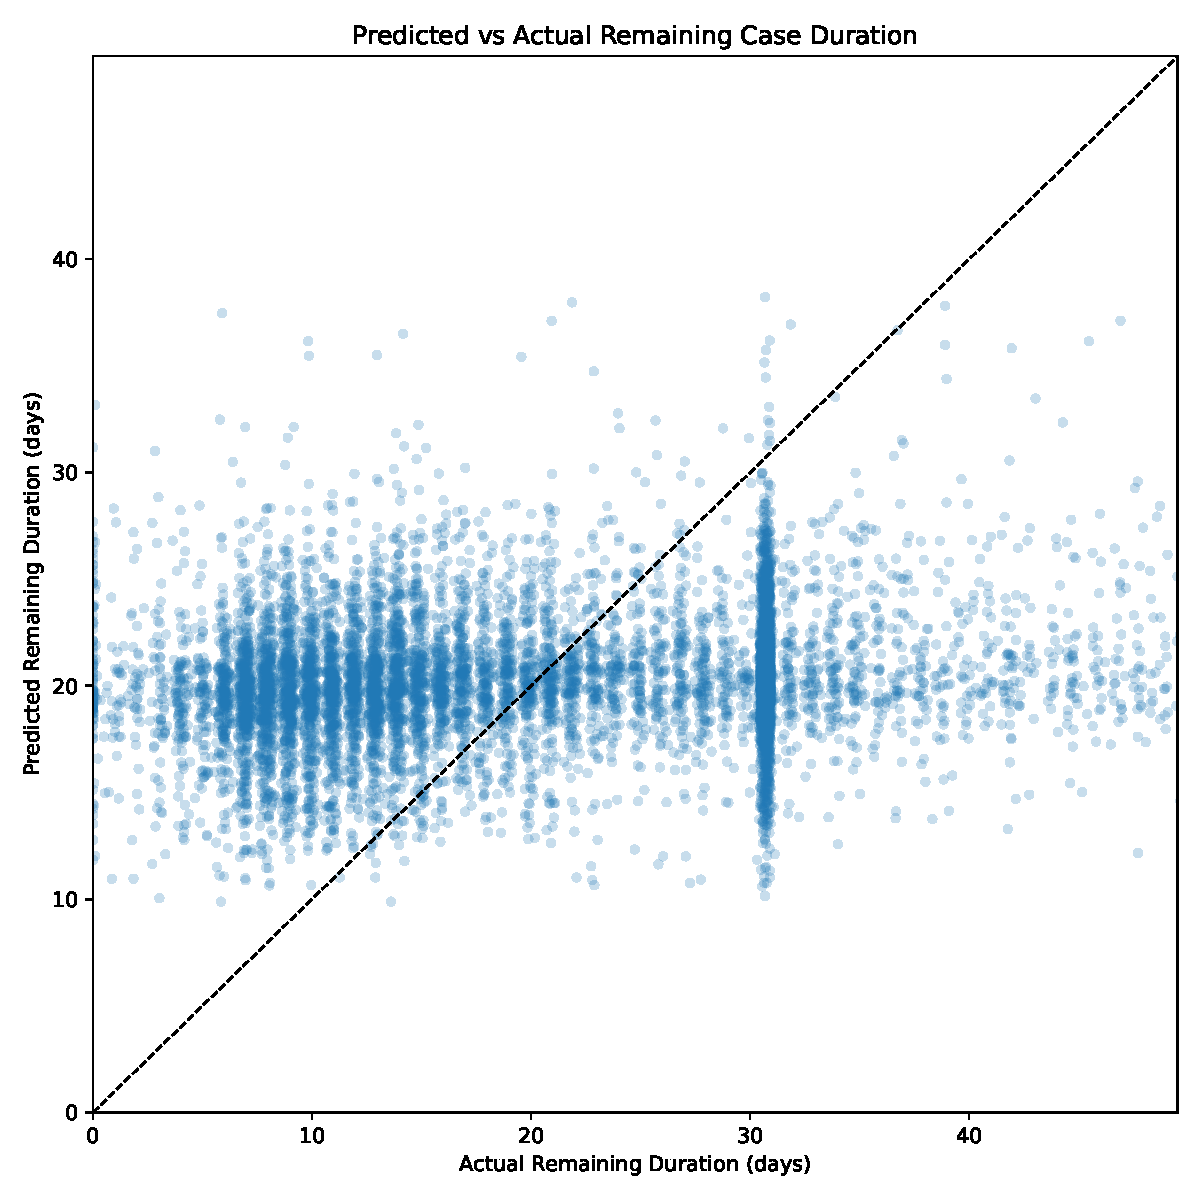
\includegraphics[width=.92\textwidth]{../figures/advanced_analysis/predicted_vs_actual_duration.pdf}
    \caption{Predicted versus actual remaining duration.}
    \label{fig:predictedactual}
\end{figure*}

\end{document}
